\documentclass[numbering=fraction]{beamer}

\usepackage[utf8]{inputenc}
\usepackage[T1]{fontenc}
\usepackage[french]{babel}
\usepackage{blindtext}
\usepackage{tikzsymbols}
\usepackage{graphicx}
\usepackage{wrapfig}
\usepackage{bookman}
\usepackage{subcaption}
\usepackage[export]{adjustbox}



\usetheme[progressbar=frametitle]{metropolis}

%Define colors
\definecolor{wuppergreen}{RGB}{85, 171, 38}
\definecolor{background}{RGB}{255,255,255}

%Adding logo to title page
\titlegraphic{\raggedleft 
\includegraphics[width=3cm]{UNamur.png}}

%Adjust color theme
\setbeamercolor{frametitle}{bg=wuppergreen}
\setbeamercolor{title separator}{fg=wuppergreen}
\setbeamercolor{footline}{fg=gray}
\setbeamercolor{progress bar}{fg=black}

%Adding footer
\setbeamertemplate{frame footer}{\insertshortauthor~(\insertshortinstitute)}

\graphicspath{ {../Images/}}

%Set parameters for title page
\title{PIMS : Sprint Review 3}
\author[PIMS]{Luis Dierick \and Gaillard Matthys \and Bouncer Yassine \and Fundu Oliver \and Anderson Rosny \and Tom Marchal }
\institute{Université de Namur}
\date{\today}

\begin{document}

\begin{frame}[plain]{}
    \maketitle
\end{frame}

\begin{frame}{Table des matières}
    \tableofcontents
\end{frame}
\section{Rappel : ce qui a déjà été fait}
\begin{frame}{Rappel}
    \begin{enumerate}
        \item \textbf{Sprint 1} :
        \begin{itemize}
            \item Enquête de terrain : cellule TICE 
            \item Enquête de terrain : professeurs : Englebert Vincent, Vice-doyenne
            \item Inspection des différentes technologies : \textit{django, sprint}
        \end{itemize}
        \item \textbf{Sprint 2} : 
        \begin{itemize}
            \item Écriture de mockups
            \item Écriture de scénarios
            \item Écriture de lexique, glossaire
            \item Inspection des différents utilisateurs
        \end{itemize}
    \end{enumerate}
\end{frame}
\section{Ce qui a été fait durant ce sprint}

\begin{frame}{Burndown chart}
    \centering
    
    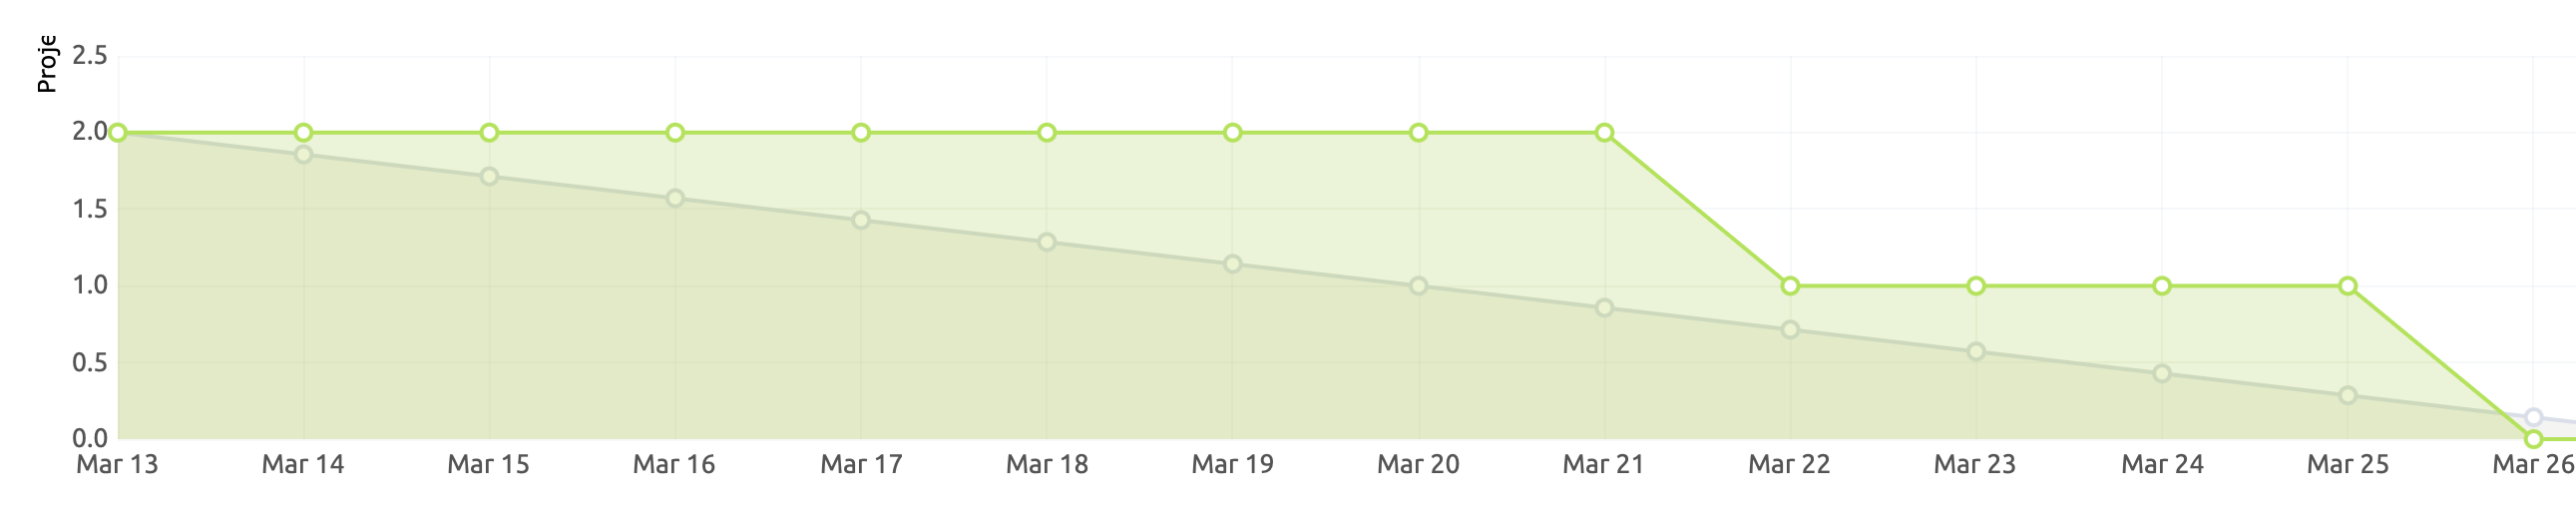
\includegraphics[width=1.1\textwidth]{burndownChart.png} 
\end{frame}

\subsection{Scénarios}
\begin{frame}{Scénarios}
    \begin{itemize}
        \item Peaufinement des mockups.
    \end{itemize}
\end{frame}

\subsection{Base de données}
\begin{frame}{Base de données}
    \begin{enumerate}
        \item Schéma de la base de données
        \begin{itemize}
            \item \textbf{Tables} : schéma entité-relation
            \item \textbf{Relationnel} : schéma relationnel
        \end{itemize}
        \item Implémentation de la base de données : 
        \begin{itemize}
            \item base de données sous postgresql
            \item conteneur docker
        \end{itemize}
        \item \textbf{Démonstration} : création de la base de données
        \begin{itemize}
            \item Script de création directement dans le conteneur
        \end{itemize}
    \end{enumerate}
    
\end{frame}
\subsubsection{Schéma entité-relation}
\begin{frame}{Schéma entité-relation}
    \begin{figure}[!ht]
        \centering
        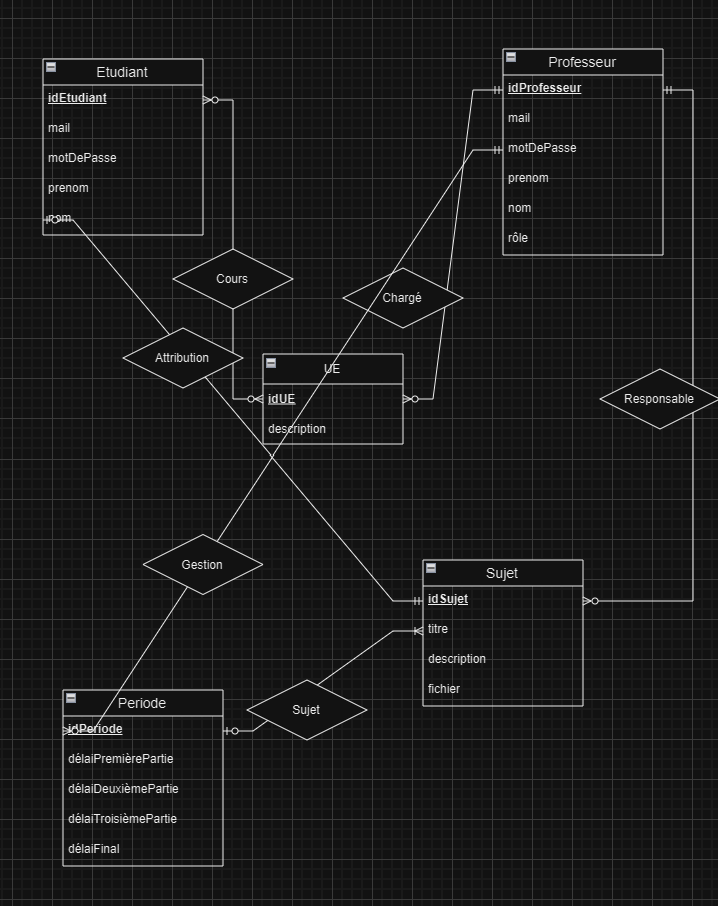
\includegraphics[scale=0.5]{entiteRelation.png}
        \caption{Schéma entité-relation}
    \end{figure}
    
\end{frame}
\subsubsection{Schéma relationnel}
\begin{frame}{Schéma relationnel}
    \begin{figure}[!ht]
        \centering
        \includegraphics[scale=0.5]{schéma relation.png}
        \caption{Schéma relationnel}
    \end{figure}
\end{frame}
    

\subsection{Implémentation du front-end}
\subsubsection{page d'accueil}
\begin{frame}{page d'accueil}
    \begin{figure}[!ht]
        \centering
        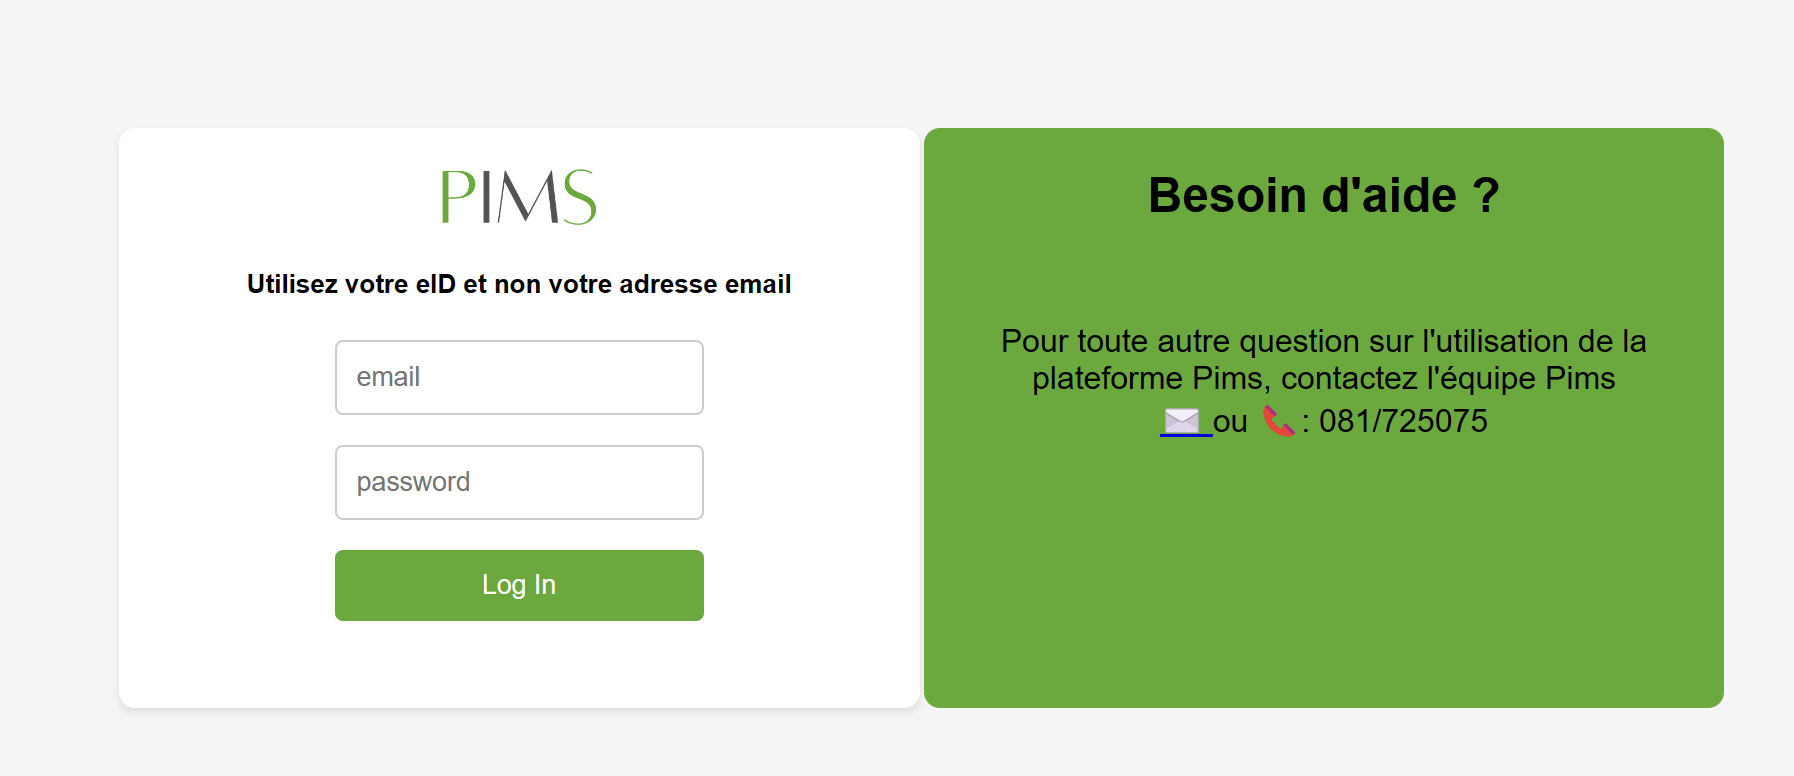
\includegraphics[scale=0.5]{pageConnexion.png}
        \caption{Page d'accueil}
    \end{figure}
\end{frame}
\subsubsection{Démonstration}
\begin{frame}{Démontration}
    \begin{enumerate}
        \item \textbf{Page d'accueil}
        \item \textbf{Choix des cours}
        \item \textbf{Ajout de sujet}
    \end{enumerate}
\end{frame}
\section{Ce qui sera fait pour le prochain sprint}
\begin{frame}{Idées}
    \begin{itemize}
        \item Avancement sur la fin des scénarios
        \item Avancement sur la fin de la base de données
        \item Avancement sur le du front-end à partir des scénarios
        \item Si possible travailler sur l'algorithme de résolution de conflit.
    \end{itemize}
\end{frame}


\end{document}